\documentclass[12pt]{article}
\usepackage[document]{ragged2e}
\pagestyle{headings}

% Layout Optimization
\usepackage{parskip}
\usepackage{multicol}

% PDF enhancement
\usepackage{hyperref}

% We use Source Han Serif TC to
% match the English font.
\usepackage{luatexja-fontspec}
\setmainjfont{Source Han Serif TC}

% Emoji
\usepackage{emoji}

% Line height
\usepackage{setspace}
\onehalfspacing

% Image
\usepackage{float}
\usepackage{graphicx}
\graphicspath{ {images/} }

\title{Personal README: A elegant readme that can be interpreted without CSS}
\author{Yi-Jyun Pan}
\date{}

\begin{document}
  % Monospace
  \newcommand{\code}[1]{\texttt{#1}}

  \maketitle

  以 GitHub 上的自介為基礎,使用 Semantic HTML、自己定義的 design system,
  以及 ES Module + TypeScript 打造出的實驗性個人介紹頁面。特色除了較為美觀的樣式外,
  還包括無 CSS 的情況下,仍然保有標準 HTML 的標題層次結構。

  \tableofcontents

  \newpage

  \section{File Hierarchy}

  有三個檔案:

  \begin{itemize}
    \setstretch{1}
    \item \code{personal-readme-src.zip}: 原始碼檔案,包含建置說明 (\code{README.md})。
    \item \code{personal-readme-dist.zip}: 可以直接開啟 index.html 閱讀的組譯後檔案。
    \item \code{readme.pdf}: 程式說明、執行結果、作業心得等。
  \end{itemize}

  \section{Tech Stack}

  \begin{itemize}
    \setstretch{1}
    \item HTML
      \begin{itemize}
        \item 使用 Semantic HTML 進行標籤。
        \item 遵守 \code{h1}, \code{h2} 等 header 定義風格,便於在無 CSS 或
        非瀏覽器環境下能夠了解網頁結構。不過 CSS 會隱藏部分
        比較累贅的 header,增加視覺乾淨程度。
      \end{itemize}
    \item SCSS
      \begin{itemize}
        \item 以 SUIT 風格 BEM 為基礎,定義元件的 class。
        \item CSS 的檔案是模組化的。
        \item Design System 以 Tailwind CSS 為基礎繼續打磨。
      \end{itemize}
    \item Scripts
      \begin{itemize}
        \item 使用 TypeScript 撰寫,配合全靜態類型定義 (\code{declare}, 無 \code{any})。
        \item 使用 ES Module 技術,且動態載入 \code{hotreload.ts} 加速網頁載入。
        \item 開發模式下,有包含啟用 Parcel Hot Reload 的 snippet。
        \item 早期版本有增強網頁功能(如 \code{u-autolink})的指令碼。
          \begin{itemize}
            \item 後期達到 0 JS 目標,\code{u-autolink} 直接替換為 \code{href}。
            \item 去除的 commit 時間點是 \code{1a2798d}。
          \end{itemize}
      \end{itemize}
    \item Bundler
      \begin{itemize}
        \item 使用開箱即用的 Parcel。
          \begin{itemize}
            \item 適合小專案,缺點是生態不足和 codebase 的潛在缺點。
            \item 大專案更建議使用 Webpack。
          \end{itemize}
        \item 根據 \code{browserslist} 定義產生出 polyfilled 的 HTML / CSS / JS dist 檔案。
        \item 壓縮等級已拉至較高等級。
      \end{itemize}
    \item Linters \& Formatters
      \begin{itemize}
        \item \code{ESLint}: 只啟用 TS code smells 檢查,沒有 enforce 程式碼風格。
        \item \code{Prettier}: 原則上採用 Prettier 預設風格。
        \item \code{Stylelint}: 除啟用 SCSS/Standard/Prettier 規則外,亦導入 SUIT BEM Pattern 的驗證。
      \end{itemize}
    \item Chores
      \begin{itemize}
        \item \code{pnpm}: Much faster than \code{npm} \& \code{yarn}.
        \item \code{fish}: Opinioned shell with elegant syntax.
        \item \code{EditorConfig}: Match the style we defined in \code{prettier} defined in VS Code.
        \item \code{Git}: Version control.
      \end{itemize}
  \end{itemize}

  \newpage

  \section{Screenshots}

  \subsection*{Desktop}
  \begin{figure}[ht]
    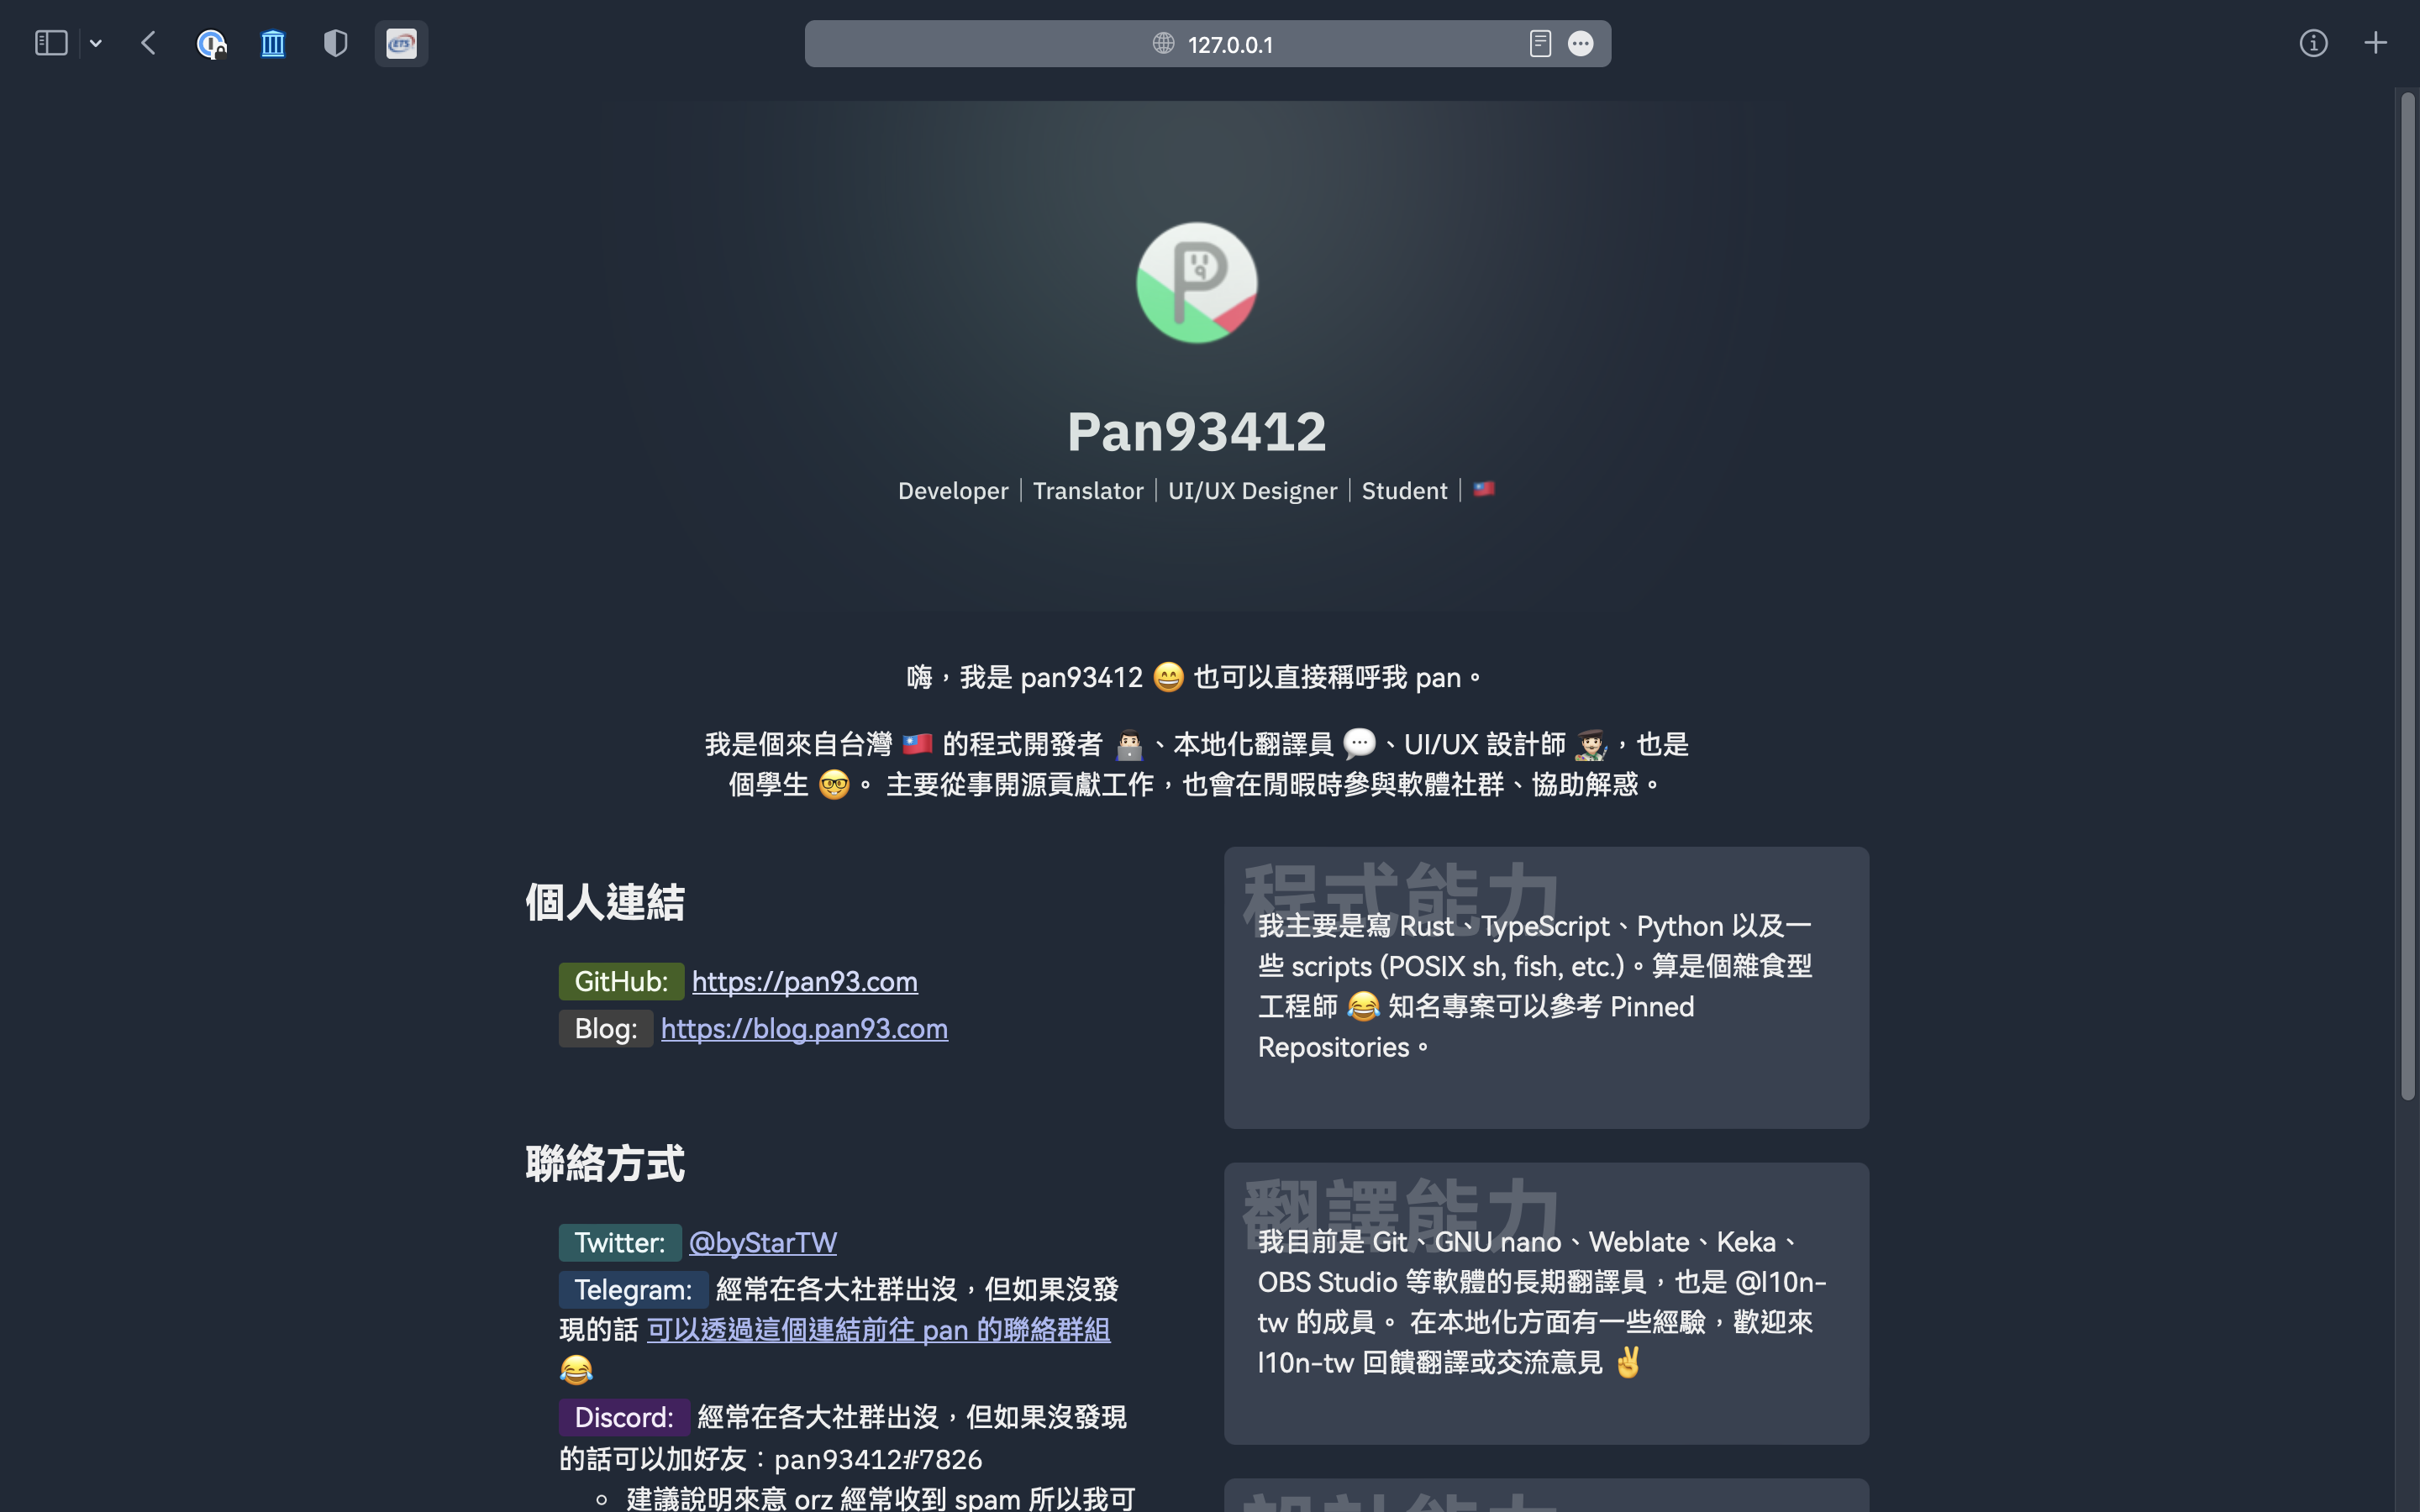
\includegraphics[width=\linewidth]{desktop.png}
  \end{figure}

  \begin{figure}[ht]
    \begin{multicols}{2}
      \subsection*{Mobile}
      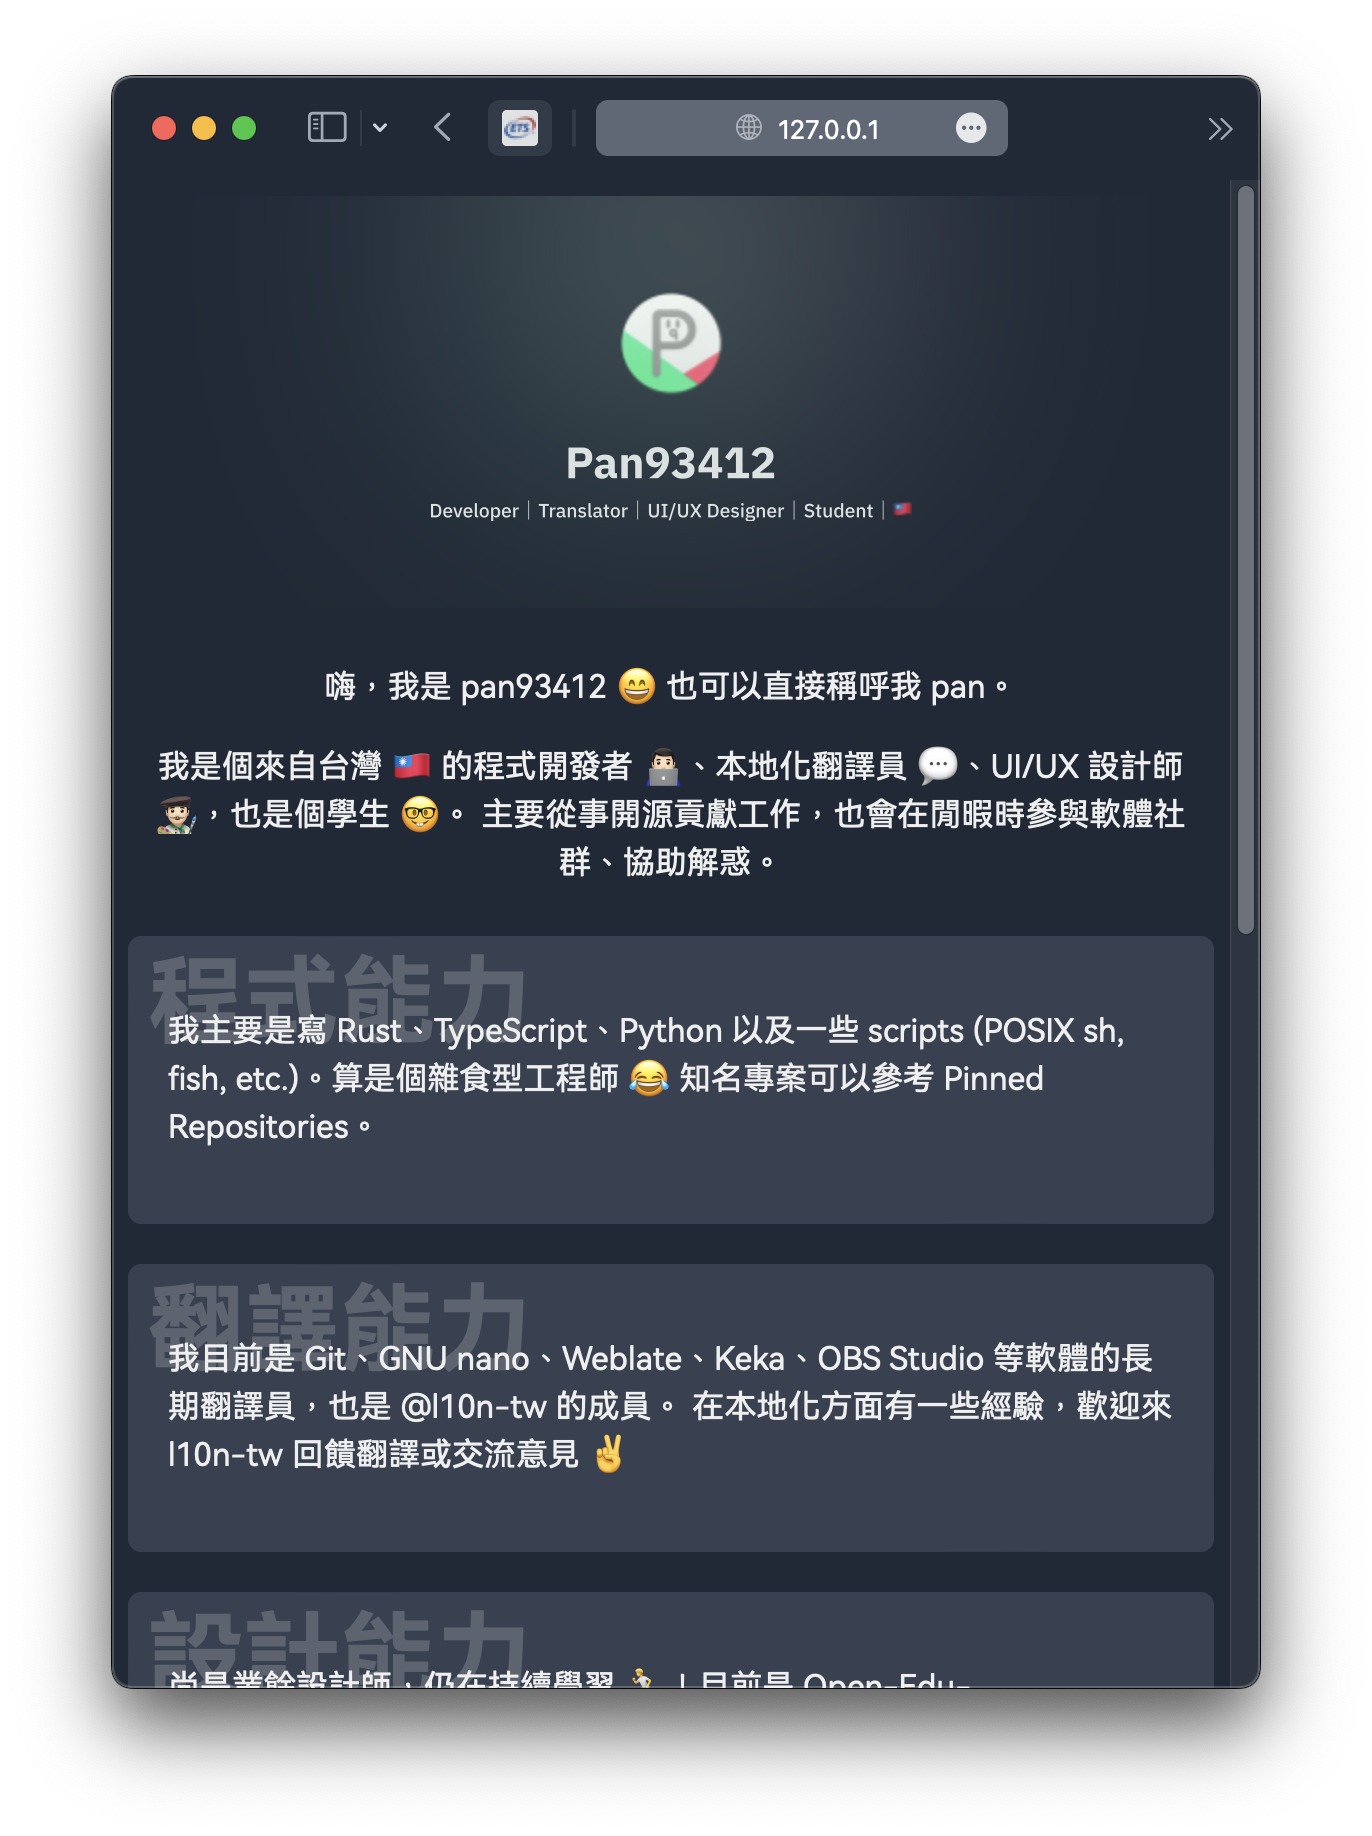
\includegraphics[width=\linewidth]{mobile.png}

      \subsection*{Mobile, without CSS}
      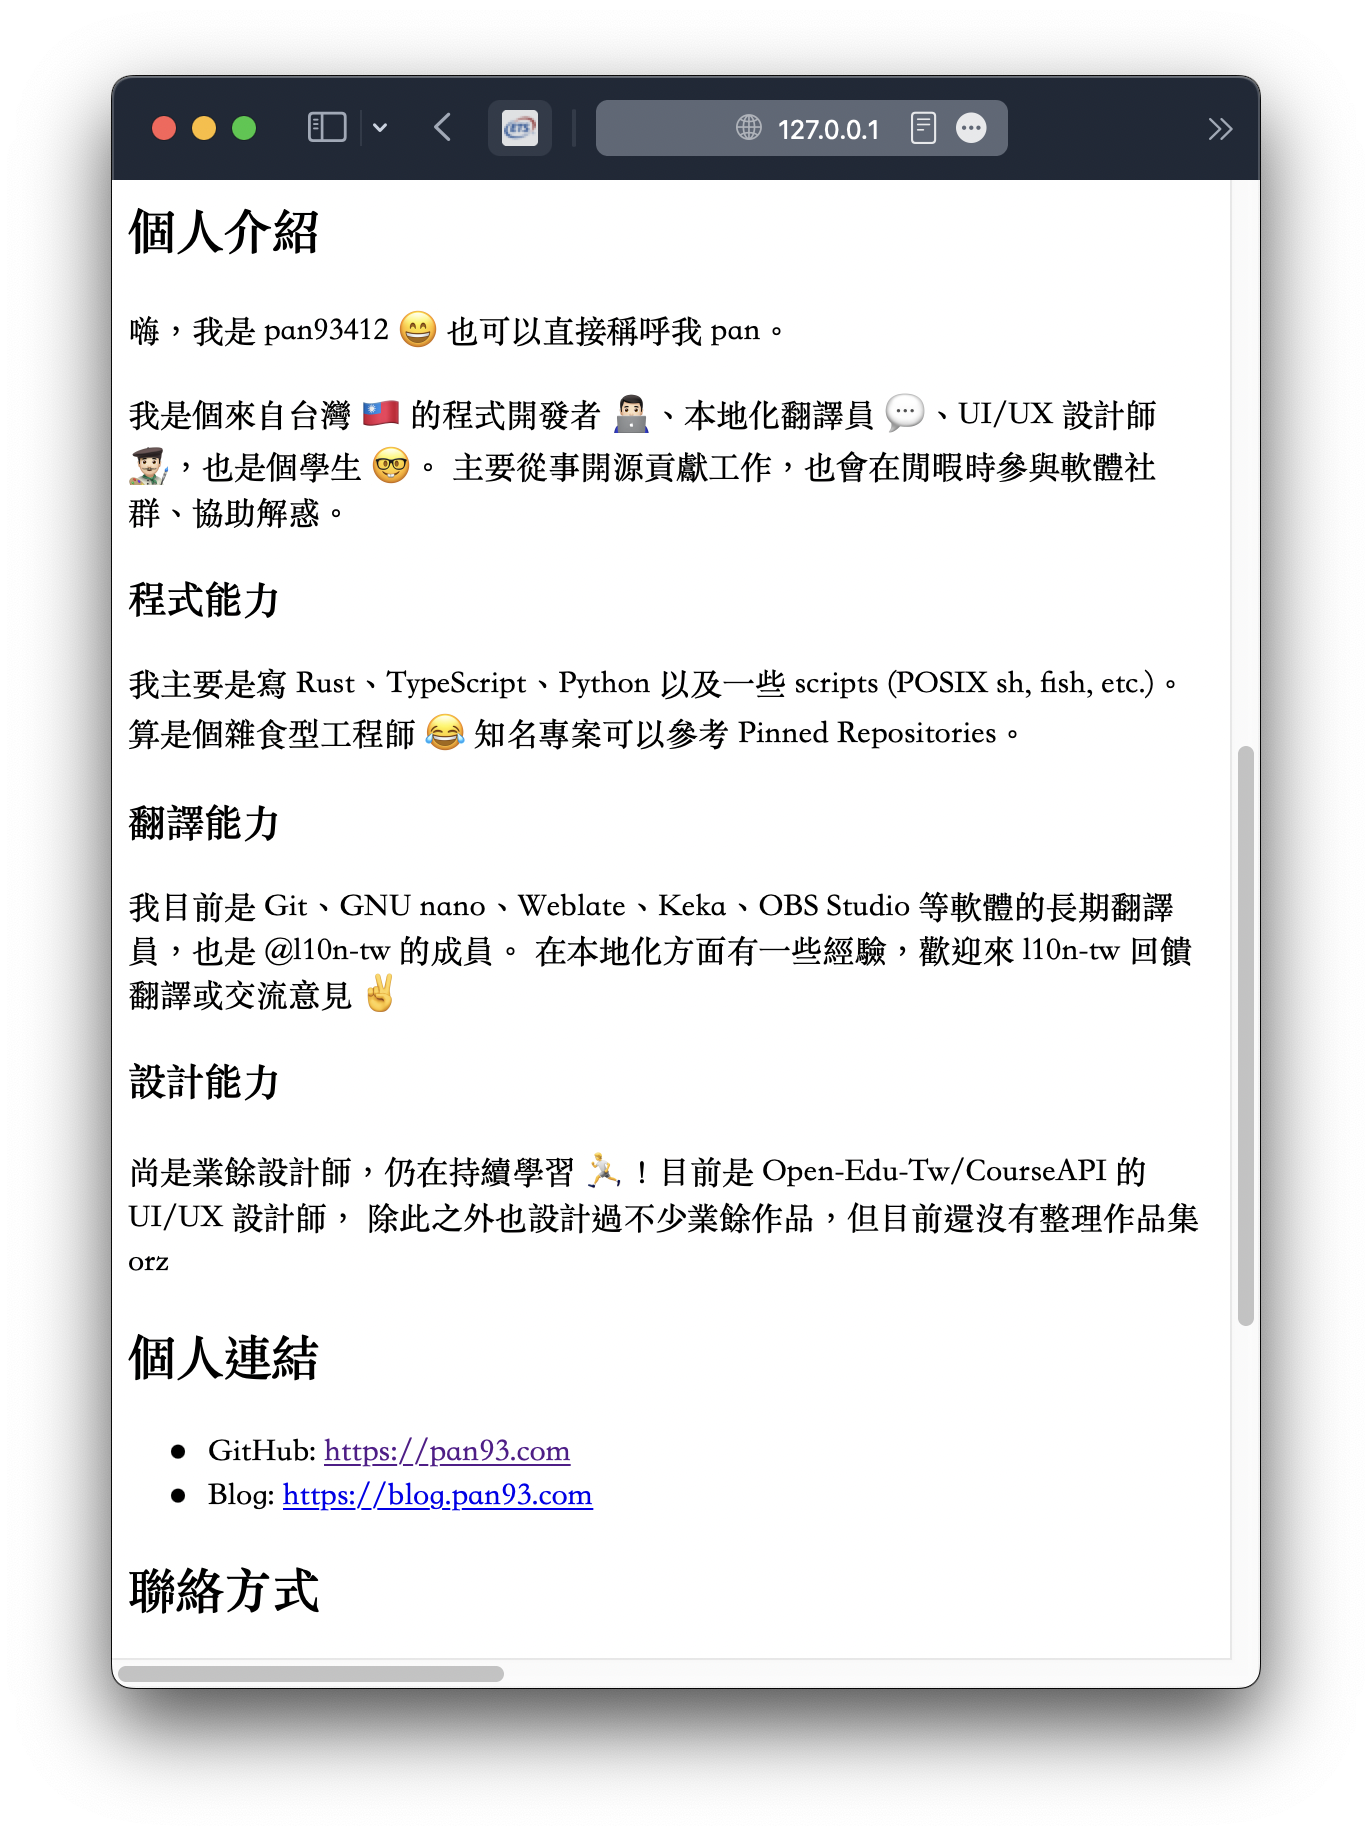
\includegraphics[width=\linewidth]{without-css.png}
    \end{multicols}
  \end{figure}

  \newpage

  \section{Reflection}

  \subsection{重新看待技術:BEM、SCSS 和 Parcel}
  自從用了 Tailwind CSS 之後,我甚少手寫 CSS。習慣了 Tailwind CSS 的
  \code{text-center flex gap-3},反而都忘記了傳統的 \code{display: flex;} 語法。

    我是在「基礎網頁設計」這堂課,看到老師介紹 \href{https://roadmap.sh/frontend}{Roadmap}
  \footnote{幫推:小克有把這個 Roadmap 比較早的版本\href{https://github.com/goodjack/developer-roadmap-chinese}{翻譯成繁體中文},也可以支持閱讀一下~},
  意外發現到一個我還沒碰過的東西:「BEM」,他是一個可以讓 CSS class name 變得整潔的 architecture。
  在此之前,我習慣這樣寫 class name(不用 Tailwind CSS 的情況下):

  \begin{verbatim}
    <nav class="navbar is-fullwidth">
      <div class="title">...</div>
      <ul class="navbar">...</ul>
      <div class="functions">...</div>
    </nav>
  \end{verbatim}

    如果用了 Tailwind CSS,那甚至不寫每個 class name 是「什麼組件」,而是
  直接把 class name 當 CSS 用了:

  \begin{verbatim}
    <nav class="w-full flex justify-between">
      <div>...</div>
      <ul class="list-none flex gap-3">...</ul>
      <div>...</div>
    </nav>
  \end{verbatim}

    這樣子的缺點是很難搞清楚「這個 \code{div} 有什麼用」,而套用 BEM
  之後,原先雜亂的架構便一目了然:

  \begin{verbatim}
    <nav class="Navbar w-full flex justify-between">
      <div class="Navbar-title">...</div>
      <ul class="Navbar-navArea list-none flex gap-3">...</ul>
      <div class="Navbar-functions">...</div>
    </nav>
  \end{verbatim}

    另外我也重持 CSS 和 preprocessor “SCSS”。寫 CSS 自由比 Tailwind CSS
  大多了——比如可以輕易做出 CSS reset,也讓樣式變得更加好讀(也更容易寫註釋)。
  而曾經因為 Parcel 的不易擴充性,我一刀斷認為 Parcel 就是不可靠的工具,並且只在
  自己的專案中使用 Webpack 和 Vite;但在這次的專案中,我發現 Parcel 在小專案
  「開箱即用」有著非常大的優勢,並對它有了正面的看法。

  \subsection{開發理念的改變:非得「best practice」嗎?}
  \begin{center}
    \textbf{很久沒寫 Vanilla JS,回到框架前的世界了。}
  \end{center}
  上次熱衷於如此「簡樸的 Tech Stack」\footnote{相對來說。其實跟很多微前端相比還是很「重」了。},
  已經是高中一年級的事情了——那時候剛入門前端不久,喜歡用 Bulma、Vanilla JS,
  不用框架地刻出一個個小工具。雖然這些小工具都不太「實用」,但卻是我前端生涯最快樂的時候:
  沒有「best practice」的約束,可以盡情地揮灑自己的想法。

    後來學了 React 和一些前端技術,並且將前端「工程化」之後,寫程式的壓力便與日俱增。
  時常會考量「是不是要 \href{https://www.componentdriven.org}{\textit{Component-Driven Development}}?」、
  「該不該導入 \href{https://nx.dev}{\textit{Monorepo}} 降低組件間的藕合度?」
  寫程式要考慮的點(技術選型)變多了,開發一個專案的壓力變大了。

    這個專案是我最近第一次嘗試「用回傳統的 HTML、CSS 和 JS 開發小 app。」
  說實話,盡情的對專案進行各種修改,而不用花很多時間在「專案配置」上,挺快樂的——
  我似乎找回了高中時對網頁開發熱情、不停嘗試各種新玩意的我。因此,這個專案的開發時長
  也算是近期專案中最長的。

    這使我省思:「究竟有沒有必要花太多時間,在『專案草創』階段就花很多時間
  在擬合所謂的『best practice』上?」彼時剛好業主把某個專案轉交給我完成,而我在這個專案中,決定不要想著要在
  「專案開始之初就配置完一切項目」——而是先從 Essential 的結構開始開發,
  再慢慢根據開發規模添入工具。事實證明這種開發模式比起之前的「配置完一切」來得比較沒有壓力,
  也可以不用一直跟組建工具抗爭。算是開發 Introduction 的另一種收穫吧。

  \newpage

  \subsection{意外的收穫:學習用 \LaTeX 撰寫這次的「動機」}
  以前就會用 \LaTeX 寫數學公式,但從來沒有用過 \LaTeX 排版。

        $$y = f(x) = ax+b$$

    而我原本是想使用 \href{https://commonmark.org}{Markdown} 來寫這次的 README,可是光 Markdown
  太單調了,輸出成 PDF 應該會比較酷,所以我花了點時間研究 \href{https://pandoc.org}{Pandoc}、
  配上 \href{https://www.overleaf.com/learn/latex/XeLaTeX}{Xe\LaTeX}、
  設定 \href{https://ithelp.ithome.com.tw/articles/10242863}{\textit{Front Matter}}……
  然而 Pandoc 輸出的內容一直不是想要的樣子(圖片錯位、排版超出文件範圍……)。
  不過,配置 Pandoc 的過程中,我突然想到:「既然 Pandoc 也是把 Markdown 編譯成 \LaTeX,
  再把 \LaTeX 編譯成 PDF,那我為何不要直接用 \LaTeX 排版呢?」

    於是,我就開始根據網路上的教學,一步步引入套件、尋找問題、撰寫內容。
  雖然 \LaTeX 的入門門檻挺高的(如何找和安裝套件、處理 CJK 字元問題 etc.),
  但處理完前置作業之後,\LaTeX 排版居然在某些情況下比 Word 還好用:
  可以輕鬆撰寫 code block、也可以做出很多程式化的自訂(比如引入組建當時的 Git commit hash)。
  即使我並沒有寫數學文件和論文的需求,之後或許也可以考慮用 \LaTeX 寫一些小文章 \emoji{joy}。

  \begin{quote}
    \textbf{後記:}後來寫 \code{utils/build-readme.fish} script 的時候,
    還遇到了很多亂七八糟的問題 \emoji{cry}。這次除了學了「怎麼寫 \LaTeX」之外,
    還學了怎麼配置 Lua\LaTeX、怎麼使用 \code{latexmk} 套件協助組建,以及一點點
    參數的使用。也算是另外的收穫吧 \emoji{joy}

    另外後期就把 Xe\LaTeX 扔掉,改用 \href{https://www.luatex.org}{Lua\LaTeX} 了。
    主要是 \href{https://tex.stackexchange.com/questions/126206/why-choose-lualatex-over-xelatex}{後者有著更好的擴充性和相容性}。
    最重要的點,是它可以使用 \code{emoji} 套件
    \emoji{partying-face}!不過缺點是編譯速度變慢了一點,
    之後再思考怎麼 optimize。
  \end{quote}

  \newpage

  \section{Source Code and License}

  \begin{itemize}
    \item GitHub: \url{https://github.com/pan93412/personal-readme-v2}
    \item License: AGPL-3.0-or-later
  \end{itemize}

  Permissions of this strongest copyleft license are conditioned on making available complete
  source code of licensed works and modifications, which include larger works using a licensed work,
  under the same license. Copyright and license notices must be preserved. Contributors provide an express
  grant of patent rights. When a modified version is used to provide a service over a network, the complete
  source code of the modified version must be made available.
\end{document}
